\chapter{Analiza tematu} \label{ch:analiza-tematu}

\section{Definicja Big Data}

Termin \english{Big Data} odnosi się do zbiorów danych o dużej objętości i specjalnych technik
opracowanych do ich przetwarzania. Ze względu na wysoki stopień personalizacji istniejących
systemów, popularne definicje tego terminu znacząco się od siebie różnią. Mimo że idea przetwarzania
ogromnych ilości danych jest wspólnym mianownikiem, różne organizacje, naukowcy i eksperci mogą
mieć odmienne podejście do definicji tego terminu w~zależności od kontekstu, w którym jest używany.

\english{Big Data} może być rozumiane jako zdolność do przetwarzania dużych zbiorów danych
w celu wyciągania wniosków ważnych dla przedsiębiorstw \cite{big-data-2}, takich jak lepsze
zrozumienie klienta, optymalizacja operacji czy tworzenie nowych produktów. Z kolei dla
naukowców termin ten może oznaczać możliwość zbierania i analizowania skomplikowanych
zestawów danych w celu badania pewnych zjawisk na skalę wcześniej nieosiągalną.

Inne definicje mogą podkreślać technologie i narzędzia wykorzystywane do transformacji danych,
takie jak klastry obliczeniowe, algorytmy analizy danych czy techniki uczenia maszynowego.
Z czasem z pojęciem \english{Big Data} skojarzono kilka cech (nazywanych powszechnie czterema "V"),
które odnoszą się do technicznych trudności związanych z~przetwarzaniem tego typu danych \cite{big-data-1}:
\begin{itemize}
      \item objętość (ang. \english{volume}) -- dane są generowane w bardzo dużych ilościach.
            Przykładowo, w mediach społecznościowych generowane są miliardy interakcji dziennie,
      \item szybkość (ang. \english{velocity}) -- dane są generowane w szybkim tempie.
            Wiele aplikacji wymaga przetwarzania tych danych w czasie rzeczywistym lub niemal rzeczywistym,
      \item różnorodność (ang. \english{variety}) -- dane napływają w różnych formatach, od
            relacyjnych baz danych do niestrukturalnych treści takich jak e-maile, zdjęcia i filmy,
      \item prawdziwość (ang. \english{veracity}) -- dane mają ograniczoną dokładność, nie wszystkie
            są przydatne, przez co ważne jest zrozumienie ich wiarygodności i dokładności.
\end{itemize}

Poza wymienionymi wyżej cechami \english{Big Data} jest często kojarzone również z wysoką rozdzielczością,
możliwością indeksowania, modyfikacji i dodawania atrybutów, niedokładnością, relacyjnym charakterem oraz
kompleksowością \cite{big-data-1}.

\section{Przetwarzanie Big Data}

W dzisiejszym świecie, w którym dane z różnych źródeł są produkowane w ogromnych ilościach,
stajemy przed wyzwaniem ich efektywnego przechowywania i przetwarzania. Społeczeństwo
generuje codziennie petabajty informacji, które muszą być analizowane, przechowywane i
przetwarzane w odpowiedni sposób \cite{big-data-2}.

Ze względu na tę ogromną objętość i szybki przyrost danych, tradycyjne metody stają się
niewystarczające. Dlatego też coraz bardziej istotne staje się korzystanie z odpowiedniego
sprzętu i oprogramowania, które są w stanie sprostać tym wyzwaniom. Jednym z~najważniejszych
kryteriów dla takich narzędzi jest ich skalowalność, czyli zdolność systemu do zwiększenia
swojej wydajności w odpowiedzi na rosnące obciążenie. Wyróżniamy skalowanie poziome i pionowe.

\subsection*{Skalowanie poziome}

Skalowanie poziome opiera się o dodawanie maszyn do istniejącego systemu w celu rozłożenia obciążenia
i zwiększenia całkowitej wydajności. W przeciwieństwie do skalowania pionowego, które polega na
ulepszaniu pojedynczej maszyny, skalowanie poziome opiera się o łączenie komputerów w klastry.

Główną zaletą skalowania poziomego jest lepsza opłacalność i elastyczność, z drugiej strony systemy
rozproszone są dalece bardziej złożone i trudniejsze w analizie.
Poniżej wymieniono kilka narzędzi używanych do realizacji obliczeń rozproszonych na zbiorach
\english{Big Data} \cite{big-data-3}:
\begin{itemize}
      \item Apache Hadoop -- platforma do przechowywania i przetwarzania danych,\newline
            oparta o system plików HDFS i model obliczeń MapReduce,
      \item Apache Spark –- platforma do przetwarzania wsadowego i strumieniowego,\newline
            wspiera obliczenia z wykorzystaniem rozproszonej pamięci współdzielonej,
      \item Apache Pig –- platforma do analizy danych oparta o system plików HDFS i klastry Apache Hadoop.
            Programy dla tej platformy tworzone są w języku Pig Latin, który oferuje wyższy poziom abstrakcji
            od programów MapReduce w języku Java.
\end{itemize}

Instalacja oprogramowania oraz konfiguracja klastra będącego przedmiotem badań to skomplikowane i
wymagające zadanie. Aby zebrać odpowiednią ilość informacji i odpowiednio ocenić wydajność systemu
kluczowe jest, aby metody zarządzania klastrem pozwalały na szybkie wprowadzanie zmian konfiguracji.

\subsection*{Skalowanie pionowe}

Skalowaniem pionowym nazywamy dodawanie zasobów do pojedynczego komputera w~celu zwiększenia jego
wydajności \cite{big-data-3}. Główną zaletą skalowania pionowego jest prostsza implementacja, która
nie narzuca kosztów związanych z konfiguracją dodatkowych maszyn i oprogramowania.

Takie rozwiązanie ma jednak swoje ograniczenia -- istnieje górny limit zasobów, które można dodać
do jednej maszyny, a odporność na awarie pojedynczego systemu może okazać się niewystarczająca
w niektórych zastosowaniach. Skalowanie pionowe można realizować poprzez wykorzystanie:
\begin{itemize}
      \item systemów wieloprocesorowych (ang. \english{Symmetric Multiprocessing, SMP}),
      \item procesorów wielordzeniowych,
      \item procesorów graficznych do obliczeń ogólnego przeznaczenia \newline
            (ang. \english{General-Purpose Compute on Graphics Processing Units, GPGPU}),
      \item programowalnych macierzy logicznych.
\end{itemize}

Wykorzystanie wymienionych metod do przyspieszania klastra \english{Big Data}
wymaga odpowiedniego doboru sprzętu oraz dogłębnego zrozumienia jego architektury. Współczesne
procesory wielordzeniowe i karty graficzne mają skomplikowane hierarchie pamięci, które
znacząco różnią się pod względem szybkości i pojemności \cite{computer-arch}. Optymalne
wykorzystanie tych hierarchii w programach będzie kluczowe dla uzyskania maksymalnej wydajności.

\section{Apache Hadoop}

Apache Hadoop to otwarte rozwiązanie do rozproszonego przechowywania i przetwarzania
dużych zbiorów danych, którego architektura została zainspirowana publikacjami firmy Google
na temat Google File System i MapReduce \cite{big-data-3}. Hadoop został zaprojektowany
do działania na klastrach złożonych z powszechnie dostępnego sprzętu, zapewniając przy
tym skalowalność i odporność na awarie.

Klastry Hadoop wykorzystują informacje o swojej topologii do planowania obliczeń
i~dzielenia danych tak, aby osiągnąć możliwie największą wydajność. Dane są zwykle
przetwarzane na tym samym komputerze, na którym są przechowywane, dzięki czemu
ograniczany jest przesył danych w obrębie klastra. \newpage

Klaster Apache Hadoop składa się z trzech głównych części:
\begin{enumerate}
      \item \english{Hadoop Distributed File System (HDFS)} –- rozproszony system plików dla
            platformy Hadoop. Pliki są dzielone na bloki (zazwyczaj o wielkości 128 MB lub 256 MB)
            i przechowywane w wielu egzemplarzach na różnych węzłach klastra (Rys. \ref{fig:hdfs}),
            zapewniając w ten sposób lokalność danych i odporność na awarie. System plików HDFS
            składa się z następujących komponentów:
            \begin{itemize}
                  \item NameNode –- węzeł zarządzający metadanymi i strukturą katalogów,
                  \item DataNode –- węzły przechowujące bloki danych i sumy kontrolne.
            \end{itemize}
      \item \english{MapReduce} –- domyślny model przetwarzania danych w Hadoop, wywodzący się
            z~systemów opracowanych przez Google. Na jego implementację w Apache Hadoop składają
            się następujące fazy (Rys. \ref{fig:mapreduce}):
            \begin{itemize}
                  \item \english{Map} –- przetwarzanie podzielonych danych wejściowych i utworzenie
                        par klucz-wartość, realizowane przez komponenty \english{Mapper},
                  \item \english{Shuffle/Sort} –- sortowanie par klucz-wartość i przesyłanie ich między węzłami,
                  \item \english{Reduce} –- łączenie wartości o tym samym kluczu, realizowane przez
                        komponenty o nazwie \english{Reducer}.
            \end{itemize}
            Użytkownicy definiują etapy \english{Map} i \english{Reduce}, natomiast etap sortowania
            dostarczany jest przez Hadoop.
      \item \english{Yet Another Resource Negotiator (YARN)} –- menedżer zasobów i system przydzielania
            zadań dla Hadoop, który pozwala wielu aplikacjom współdzielić zasoby w~jednym środowisku.
            Składa się z trzech typów węzłów:
            \begin{itemize}
                  \item ResourceManager –- odpowiedzialny za alokację zasobów w klastrze,
                  \item ApplicationMaster –- zarządza pojedynczym zadaniem oraz śledzi jego postęp,
                  \item NodeManager -– zarządza pojedynczym węzłem wykonawczym, komunikuje informacje
                        o dostępnych zasobach.
            \end{itemize}
\end{enumerate}

\begin{figure}
      \centering
      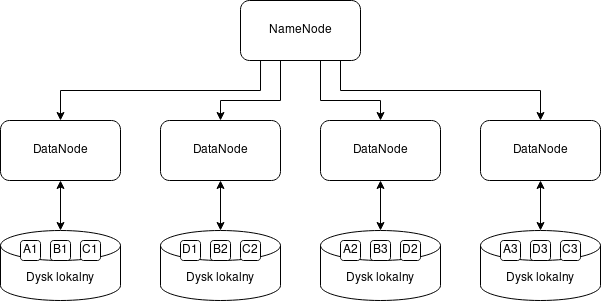
\includegraphics[width=0.7\textwidth]{./graf/HDFS.png}
      \caption{Schemat systemu plików HDFS}
      \label{fig:hdfs}
\end{figure}

\begin{figure}
      \centering
      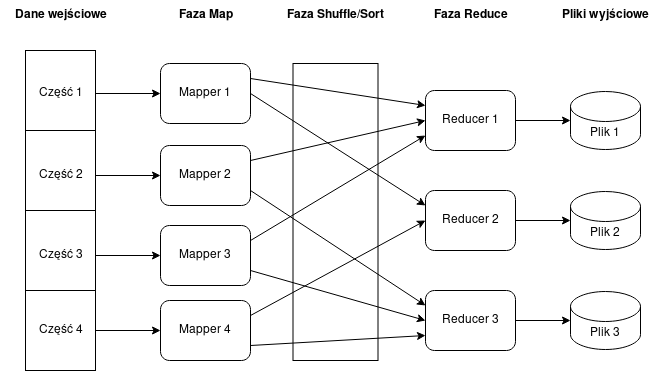
\includegraphics[width=0.8\textwidth]{./graf/MapReduce.png}
      \caption{Schemat przykładowego programu \english{MapReduce}}
      \label{fig:mapreduce}
\end{figure}

Choć implementacje faz \english{Map} i \english{Reduce} są pisane głównie w języku Java, to
narzędzie \english{Hadoop Streaming} pozwala na użycie dowolnego programu, który komunikuje się
za pomocą standardowych strumieni wejścia/wyjścia. Wskutek tego możliwe jest tworzenie
komponentów \english{Mapper} oraz \english{Reducer} w dowolnym języku programowania.

Hadoop i model MapReduce zostały zaprojektowane głównie dla aplikacji wsadowych, co oznacza,
że są lepiej przystosowane do przetwarzania dużych, zamkniętych zbiorów danych niż do ciągłego
przetwarzania strumieniowego lub iteracyjnego.

\section{Apache Spark}

Apache Spark to otwarta platforma do rozproszonego przetwarzania dużych zbiorów danych,
która oferuje wsparcie dla programów wsadowych, obróbki danych w czasie rzeczywistym,
interaktywnej analizy danych i uczenia maszynowego. Spark został opracowany w celu pokonania
ograniczeń wynikających z szybkości dysków twardych.

Platforma Spark jest oparta o struktury danych \english{Resilient Distributed Dataset (RDD)}.
Są to obiekty przechowywane w pamięci węzłów klastra w wielu egzemplarzach, które mogą być
przetwarzane równolegle. Ich użycie pozwala na nawet stukrotne przyspieszenie w porównaniu z
systemami opartymi o Apache Hadoop, zachowując jednocześnie wysoką odporność na awarie \cite{big-data-3}.

Spark zapewnia wsparcie dla wielu źródeł danych. Są to między innymi HDFS, bazy Apache
Cassandra, relacyjne bazy danych SQL i źródła Amazon S3. System ten wspiera też wiele
języków programowania, są to na przykład Scala, Python, Java oraz R.

Klaster Apache Spark może działać niezależnie, w połączeniu z systemem plików HDFS lub
z innymi systemami zarządzania klastrem:
\begin{itemize}
      \item YARN -- menedżer zasobów dla platformy Apache Hadoop,
      \item Apache Mesos -- menedżer klastra zgodny z Hadoop oraz Spark,
      \item Kubernetes -- platforma do wdrażania i skalowania aplikacji kontenerowych.
\end{itemize}

\subsubsection*{Spark SQL}

Moduł Spark SQL umożliwia przetwarzanie danych w formacie tabelarycznym przy użyciu języka
SQL \cite{spark-sql}. Spark SQL zapewnia też dostęp do danych z Apache Hive i interfejsy
dostępu do relacyjnych baz danych (JDBC oraz ODBC), co ułatwia integrację z~istniejącymi
aplikacjami.

Jednym z kluczowych elementów Spark SQL jest DataFrame, czyli rozproszona kolekcja danych
zorganizowana w kolumny. DataFrame można przyrównać do tabeli w relacyjnej bazie danych,
ponieważ wspiera on wykonywanie operacji takich jak wybieranie, filtrowanie czy agregacja.

Wraz z DataFrame pojawiły się także struktury Dataset, które łączą zalety RDD i~DataFrame,
oferując zarówno typowanie statyczne, jak i operacje na poziomie kolumn. Dataset to kolekcja
obiektów określonego typu, co oznacza, że błędy związane z typami mogą być wykrywane w czasie
kompilacji, a nie tylko podczas wykonania.

Statyczne typowanie zapewnia większe bezpieczeństwo i pewność podczas pisania kodu w
porównaniu do operacji wykonywanych na DataFrame'ach, które są typowane dynamicznie.
Przykład wykorzystania Dataset pokazano na listingu \ref{lst:spark-sql}.
\newpage

%TC:ignore
\begin{lstlisting}[
    language=Java,
    label=lst:spark-sql,
    caption={Przykładowy program wykorzystujący moduł Spark SQL.}
]
public class SparkSQLExample {

    public static void main(String[] args) {
        SparkSession spark = SparkSession.builder()
            .appName("Spark SQL w Javie")
            .master("local")
            .getOrCreate();

        // Wczytanie danych z pliku CSV
        Dataset<Row> df = spark.read()
            .option("header", "true")
            .option("inferSchema", "true")
            .csv("osoby.csv");

        // Utworzenie widoku tymczasowego
        df.createOrReplaceTempView("osoby");

        // Wykonanie zapytania SQL
        Dataset<Row> wynik = spark.sql(
            "SELECT imie, wiek FROM osoby WHERE wiek > 25"
        );
        wynik.show(); // Pokazanie wyniku w konsoli
        spark.stop();
    }
}
\end{lstlisting}
%TC:endignore

Catalyst to optymalizator używany przez Spark SQL, który optymalizuje zapytania SQL na dwóch
poziomach: najpierw na poziomie planu logicznego, następnie na poziomie planu fizycznego
\cite{spark-sql-catalyst}. Plan logiczny opisuje tylko etapy potrzebne do obliczenia wyniku,
nie uwzględniając jednak struktury klastra. Informacje te posiada plan fizyczny, który składa
się z optymalnych struktur RDD i algorytmów, dopasowanych do konkretnego klastra Spark.

Ważną cechą optymalizatora Catalyst jest oddzielenie optymalizacji od logiki zapytania. Taki
podział ułatwia wdrażanie aktualizacji i modyfikacji, a same optymalizacje mogą być używane
w wielu zapytaniach jednocześnie, co wpływa korzystnie na długoterminowe utrzymanie całego
systemu. Co więcej, optymalizacje są dobierane dynamicznie, dzięki czemu to samo zapytanie
może być wykonywane optymalnie na klastrach o różnych rozmiarach, topologiach czy
dostępnych zasobach.

\section{Architektura CUDA}

CUDA (ang. \english{Compute Unified Device Architecture}) to jedna z najbardziej popularnych
równoległych architektur dla procesorów graficznych, opracowana przez firmę NVIDIA.

Architektura CUDA realizuje model SIMT \cite{computer-arch} (ang. \english{Single Instruction, Multiple Threads},
jedna instrukcja -- wiele wątków), który łączy zalety wielowątkowości i instrukcji wektorowych.
Podstawowym elementem tego modelu jest wątek CUDA, czyli najmniejsza jednostka obliczeń, która
może być niezależnie zaplanowana do wykonania przez procesor.

Podobnie jak w modelu SIMD (ang. \english{Single Instruction, Multiple Data}, jedna instrukcja -- wiele danych),
w architekturze CUDA instrukcje są wykonywane równolegle na wielu danych. Z drugiej strony,
w modelu SIMT każdy wątek posiada własny kontekst, składający się ze stosu i rejestrów.

Wątki CUDA są zorganizowane w grupy zwane blokami (Rys. \ref{fig:cuda-grid}), w których obrębie
mogą wymieniać się danymi przez pamięć współdzieloną i synchronizować się za pomocą
barier. Zarówno bloki wątków, jak i siatki składające się z tych bloków mogą być organizowane na
różne sposoby przy użyciu struktur jedno-, dwu- lub trójwymiarowych. Ta elastyczność pomaga w
tworzeniu wydajnych programów, które pozostają proste i łatwe w utrzymaniu.

\begin{figure}
      \centering
      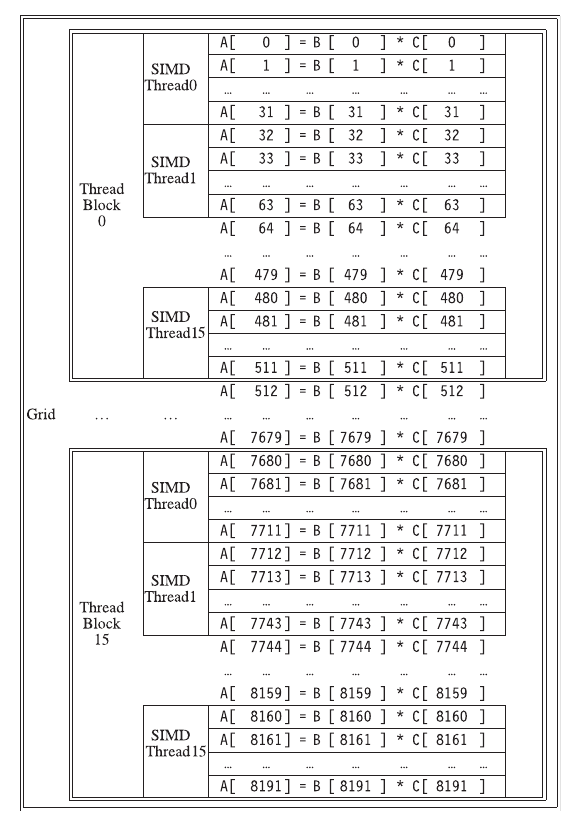
\includegraphics[width=0.8\textwidth]{graf/CUDA-Grid.png}
      \caption {
            Podział przykładowego programu CUDA na siatkę (ang. \english{grid}),
            bloki wątków (ang. \english{thread block}) i wątki CUDA (ang. \english{thread}).
            \cite{computer-arch}
      }
      \medskip \small
      Program mnoży elementy tablic B i C, wynik jest zapisywany do tablicy A.
      \label{fig:cuda-grid}
\end{figure}

W architekturze CUDA hierarchia pamięci odgrywa kluczową rolę w efektywnym wykorzystaniu
układów graficznych. Model programowania CUDA udostępnia następujące rodzaje pamięci:
\begin{itemize}
      \item rejestry -- najszybsza dostępna pamięć, używana przez pojedyncze wątki, przechowuje
            zmienne lokalne. Liczba dostępnych rejestrów jest ograniczona i zależy od generacji procesora CUDA.
      \item pamięć współdzielona -- szybka pamięć procesora, dostępna dla wątków w obrębie jednego bloku.
            Ma ograniczoną pojemność, ale dostęp do niej jest znacznie szybszy niż do pamięci globalnej.
            Aby zapewnić maksymalną wydajność, ważne jest unikanie konfliktów banków tej pamięci.
      \item pamięć globalna -- zewnętrzna pamięć procesora, dostępna dla wszystkich bloków i~wątków.
            Jest największa pod względem pojemności, ale jednocześnie ma najwyższe opóźnienia dostępu.
            Wspiera dostępy łączone, które znacznie przyspieszają operacje czytania oraz zapisu.
      \item pamięć stałych -- specjalny segment pamięci globalnej o ograniczonej pojemności, który
            jest przechowywany w pamięci podręcznej. Przeznaczony dla parametrów funkcji oraz danych,
            które nie zmieniają się podczas wykonywania programu. \newpage
      \item pamięć tekstur -- zoptymalizowana dla specyficznych wzorców dostępu, typowych dla programów
            związanych z grafiką komputerową. Dane podlegają przechowywaniu w~pamięci podręcznej procesora.
      \item pamięć lokalna -- segment pamięci globalnej, który jest używany do przechowywania zmiennych
            lokalnych wątku, gdy przekroczy on dostępną liczbę rejestrów. Charakteryzuje się większymi
            opóźnieniami od pamięci współdzielonej, ponieważ jest fizycznie przechowywana w zewnętrznej pamięci DRAM.
\end{itemize}


Układy graficzne firmy NVIDIA oferują jednakowy model programowania i wykorzystują wspólny pakiet narzędzi
programistycznych, co ułatwia tworzenie przenośnych programów. Częścią modelu programowania jest język
programowania CUDA \cite{cuda-by-example}, który jest w istocie rozszerzeniem języka C++ o hierarchiczny
model pamięci urządzenia, funkcje do synchronizacji wątków, typy wektorowe oraz możliwość definiowania
funkcji wykonywanych na procesorze graficznym, określanych też jako \english{kernel}.

Kod napisany w języku CUDA może być kompilowany do przenośnego kodu pośredniego PTX
(ang. \english{Parallel Thread Execution}), co umożliwia jego późniejszą optymalizację i wykonanie
na urządzeniach o różnych wersjach architektury CUDA.

Dzięki szerokiej dostępności bibliotek, programy CUDA mogą być wywoływane także z poziomu
innych języków, takich jak Python, Java, MATLAB oraz Rust. Niektóre narzędzia, takie jak CudaPy
dla języka Python, pozwalają też na automatyczne tłumaczenie funkcji na kod CUDA.

\section{Standard OpenCL}

OpenCL (ang. \english{Open Computing Language}) to otwarty standard umożliwiający tworzenie programów
wykorzystujących akcelerację sprzętową, w tym różnorodne kombinacje procesorów głównych, graficznych oraz
innych akceleratorów \cite{opencl}.

W porównaniu z technologią CUDA, której rozwojem kieruje NVIDIA, OpenCL został stworzony przez konsorcjum
Khronos Group określające jedynie specyfikację interfejsów. Dostarczenie odpowiednich sterowników i
implementacji OpenCL jest z kolei zadaniem należącym do producenta sprzętu.

Ze względu na otwartość tego standardu, OpenCL umożliwia pisanie kodu, który może być łatwo przenoszony i
dostosowywany do różnych architektur i platform sprzętowych. Pozwala to na większą elastyczność w projektowaniu
systemów prowadzących obliczenia.

Jednostka obliczeń (ang. \english{work-item}), odpowiadająca wątkowi w modelu CUDA, stanowi najmniejsze
możliwą do zaplanowania i wykonania zadanie. Tak jak w modelu CUDA, jednostki obliczeń mogą być organizowane
w grupy robocze (ang. \english{workgroup}), które są odpowiednikami bloków wątków. 

Komunikacja w obrębie grupy roboczej jest realizowana poprzez pamięć lokalną. Mechanizmy synchronizacji, takie jak bariery, pozwalają
na koordynację wykonania jednostek w ramach grupy roboczej.

OpenCL oferuje programistom złożony, ale jednakowy dla wszystkich urządzeń model pamięci. Jego hierarchiczna
struktura składa się z następujących elementów:
\begin{itemize}
      \item pamięć prywatna -- pamięć dostępna tylko dla jednej jednostki obliczeń. Dane w pamięci prywatnej nie
            są dostępne dla innych jednostek wykonawczych. Zazwyczaj jest używana do przechowywania zmiennych
            lokalnych w funkcjach. Jest to ekwiwalent pamięci lokalnej w CUDA.
      \item pamięć lokalna -- dostępna dla wszystkich jednostek obliczeń w obrębie jednej grupy roboczej. Jest szybsza
            niż pamięć globalna i idealnie nadaje się do przechowywania tymczasowych danych. Podobna do pamięci
            współdzielonej w modelu CUDA.
      \item pamięć globalna -- pamięć dostępna dla wszystkich jednostek obliczeń w~obrębie kernela. Ze względu
            na jej globalny charakter, dostęp do niej może być wolniejszy w~porównaniu z innymi rodzajami pamięci,
            dlatego jej użycie powinno być ograniczane. Jest odpowiednikiem pamięci globalnej w CUDA.
      \item pamięć stałych -- specjalny segment pamięci globalnej, który może być odczytywany przez jednostki
            obliczeń. Na niektórych urządzeniach jest to część pamięci podręcznej. Odpowiednik pamięci stałych w CUDA.
\end{itemize}

Ze względu na konieczność zapewnienia wsparcia dla różnych typów procesorów, model pamięci OpenCL nie
zawiera pamięci tekstur, pozwalającej na optymalizację wzorców dostępu typowych dla aplikacji grafiki komputerowej.

Oprócz modelu obliczeń i pamięci, OpenCL opisuje też języki programowania przeznaczone dla
akceleratorów. Są to języki oparte o standardy C99, C++14 i C++17, rozszerzające je o funkcje
związane z zarządzaniem pamięcią, synchronizacją jednostek obliczeń oraz operacjami wektorowymi.

Podobnie jak w przypadku języka CUDA, kod OpenCL może być kompilowany do reprezentacji pośredniej.
W przypadku OpenCL jest to SPIR (ang. \english{Standard Portable Intermediate Representation}),
który przed wykonaniem programu jest optymalizowany dla architektury konkretnego urządzenia.
\newpage

\section{Klastry oparte o minikomputery jednopłytkowe}

Klastry obliczeniowe zbudowane z komputerów jednopłytkowych cechują się dużą skalowalnością.
Dobrym przykładem są systemy zbudowane przez firmy Balena i Oracle, które służą głównie jako
demonstratory technologii do rozproszonego przechowywania danych i~zarządzania serwerami,
składają się zatem z setek lub nawet tysięcy węzłów.

Klaster Beast v2 został skonstruowany przez firmę Balena jako następca wcześniejszej wersji,
Beast v1. Składa się on ze 144 minikomputerów Raspberry Pi 3B, połączonych siecią Gigabit
Ethernet. Konstrukcja ukazana na rysunku \ref{fig:balena-cluster} osiąga wysokość 2 metrów
i~masę około 150 kilogramów.

Klaster był pierwotnie przeznaczony do testowania i demonstracji oprogramowania resin.io,
a ostatecznie został wysłany do klienta, który sponsorował jego budowę. Wkrótce potem
rozpoczęto projektowanie kolejnej iteracji, nazwanej "Beast v3", która ma na celu dalsze
zwiększenie modułowości, gęstości i łatwości montażu \cite{balena-cluster}.

\begin{figure}[h]
      \centering
      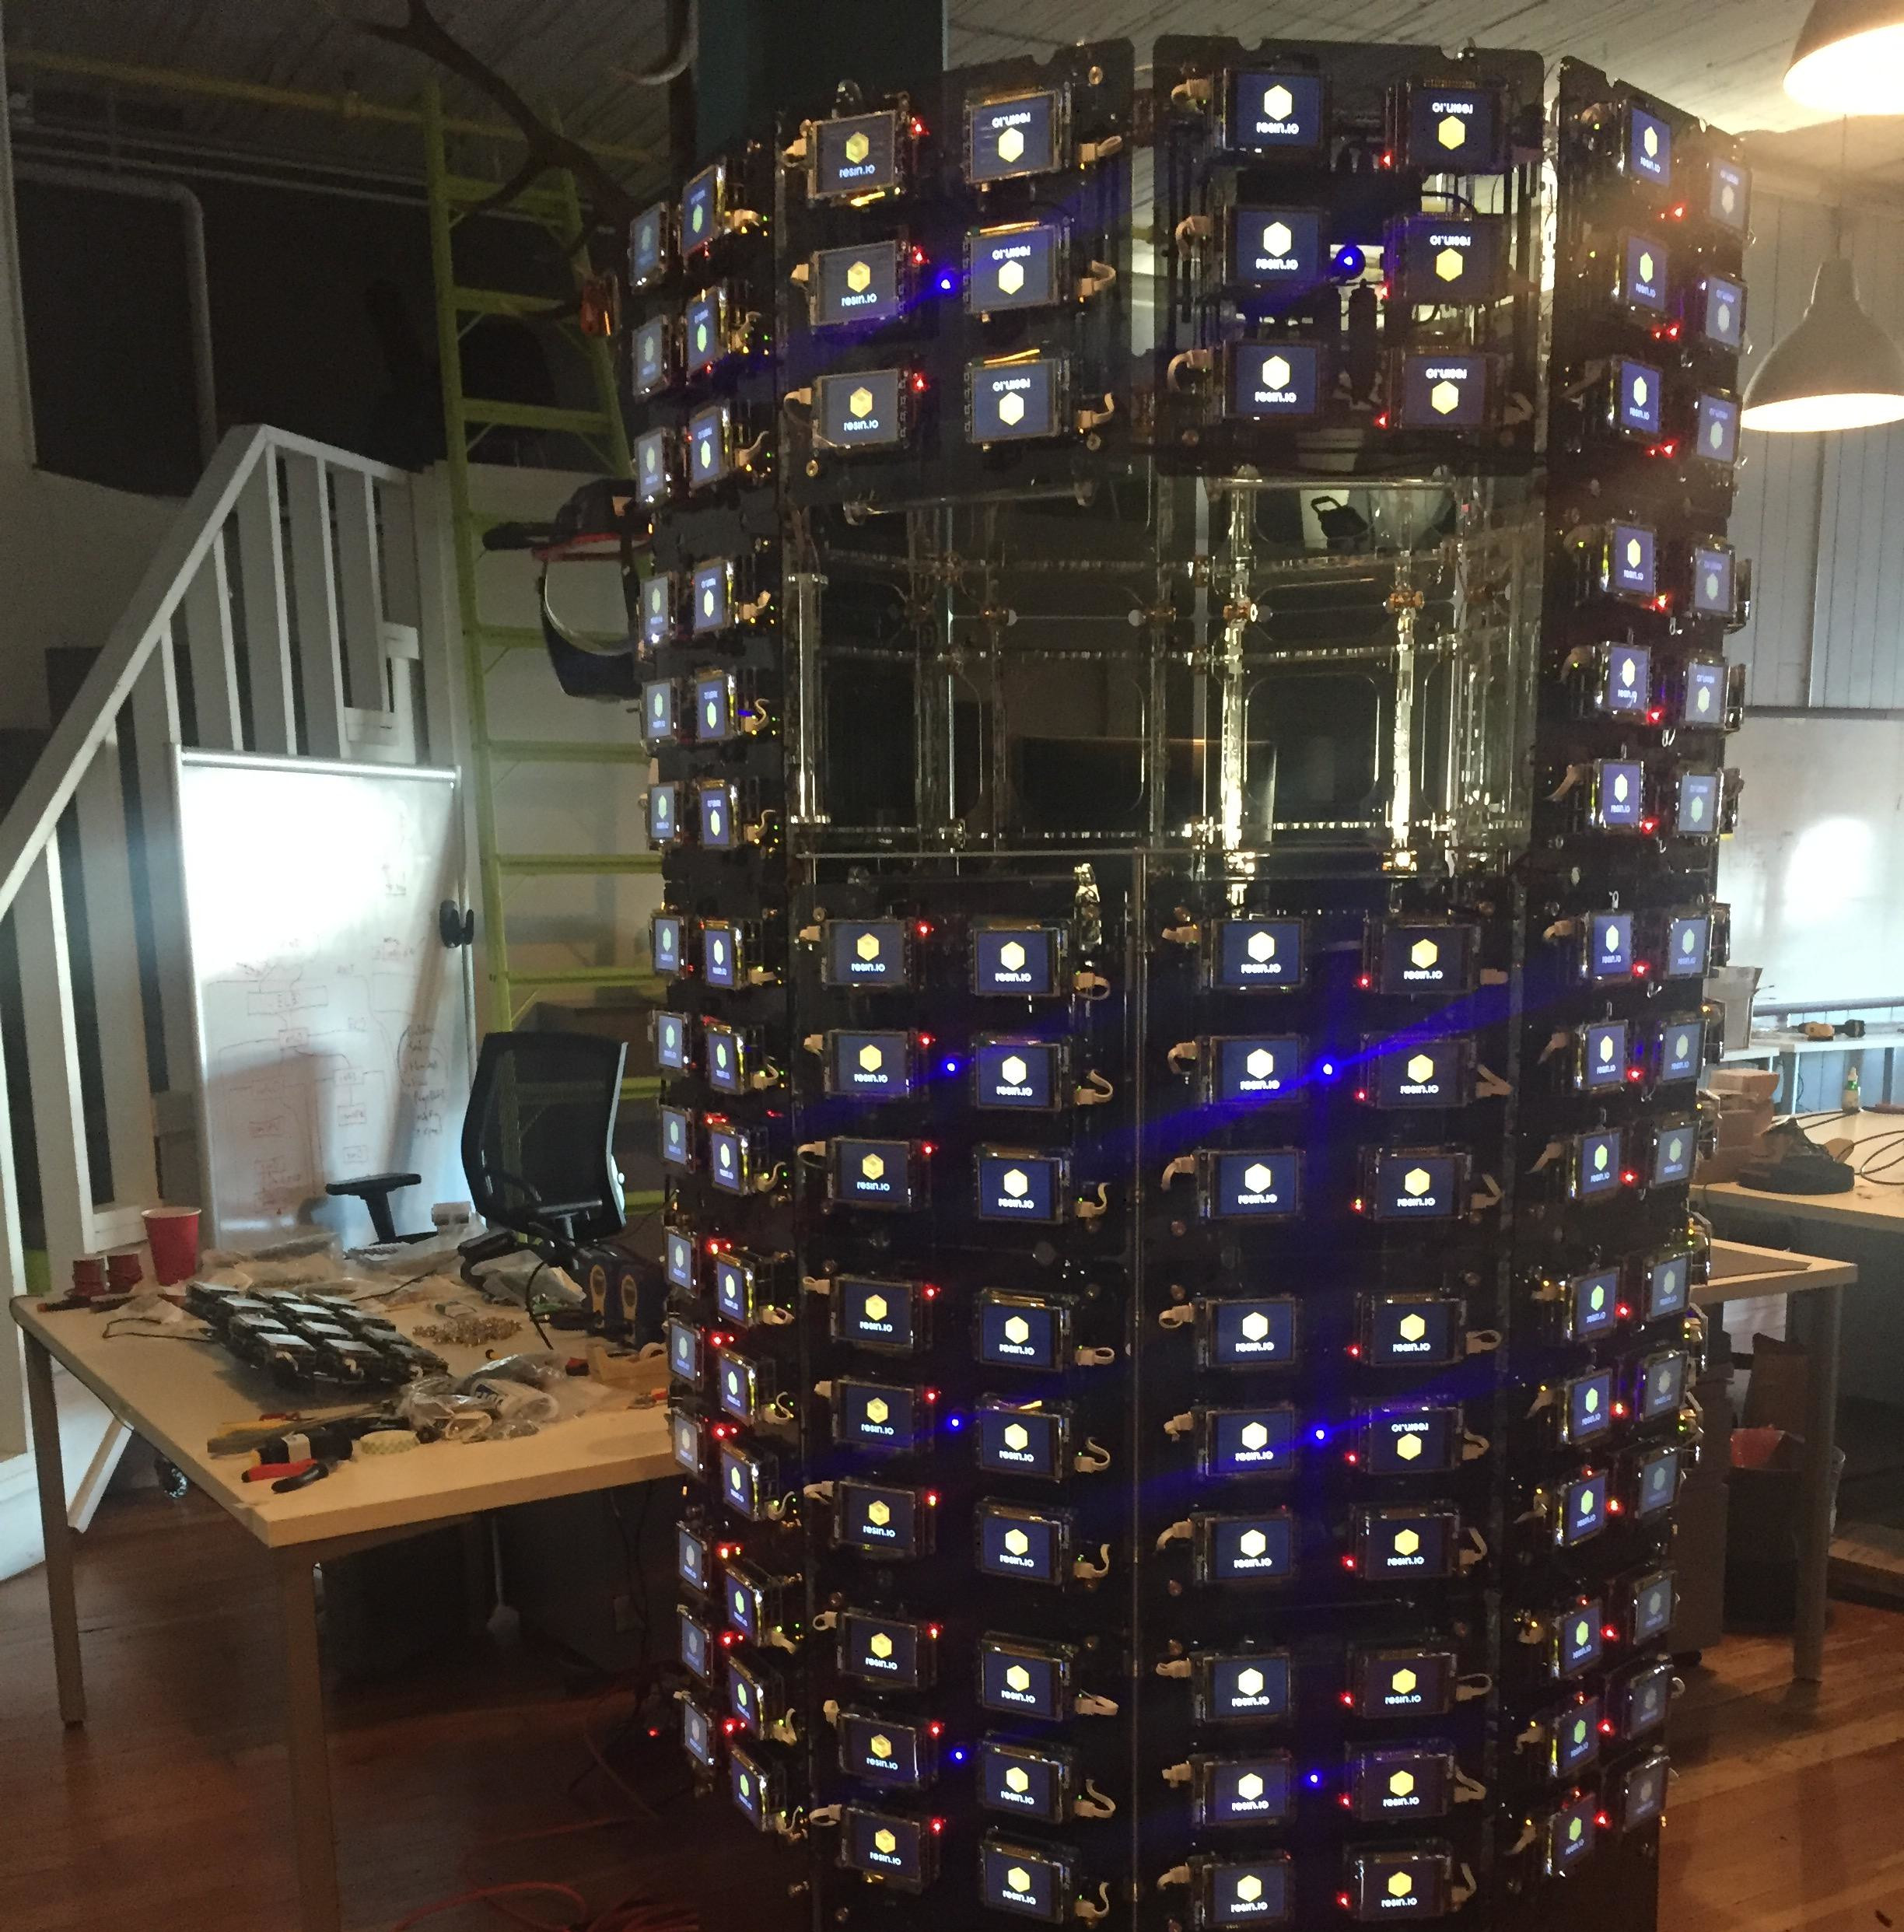
\includegraphics[width=0.9\textwidth]{graf/Balena.jpg}
      \caption {
            Klaster Beast v2. \cite{balena-cluster}
      }
      \label{fig:balena-cluster}
\end{figure}

System firmy Oracle, nazwany \english{Raspberry Pi Supercomputer}, został zaprezentowany po raz
pierwszy na targach OpenWorld 2019 (Rys. \ref{fig:oracle-cluster}). Składa się on z 1060
minikomputerów Raspberry Pi 3B+ umieszczonych w szafach 2U, gdzie każda półka mieści 21 węzłów.
Węzły zostały połączone za pomocą sieci w standardzie Gigabit Ethernet.

Komputery Raspberry Pi zostały umieszczone w obudowach wykonanych w technologii druku 3D.
Zasilanie węzłów jest zapewniane przez zasilacze USB, które zostały wybrane ze względu na
mniejszy koszt i większą sprawność w porównaniu do zasilania przez interfejsy Ethernet
(ang. \english{Power over Ethernet, PoE}). Wdrożenie Oracle Linux zostało przeprowadzone
za pomocą centralnego serwera rozruchowego \cite{oracle-cluster-1}.

Przedstawiony klaster pokazał możliwości dystrybucji Oracle Linux, języka programowania Java
oraz bazy danych Oracle w kontekście integracji powszechnie dostępnych komponentów, takich jak
Raspberry Pi, w klastry obliczeniowe dużego formatu \cite{oracle-cluster-2}.

\begin{figure}[h]
      \centering
      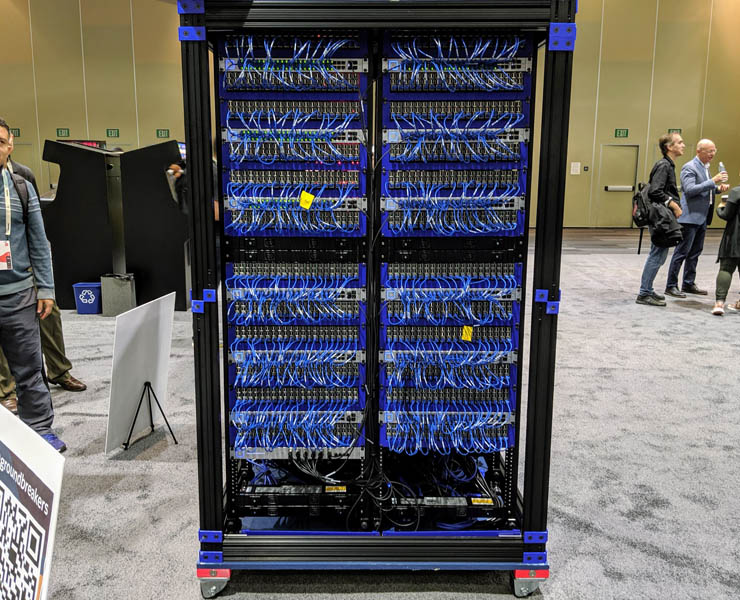
\includegraphics[width=0.9\textwidth]{graf/Oracle.jpg}
      \caption {Klaster Raspberry Pi Supercomputer firmy Oracle. \cite{oracle-cluster-1}}
      \label{fig:oracle-cluster}
\end{figure}

Artykuł autorstwa A. Neto, J. Neto i E. Moreno \cite{rpi-cluster-1} opisuje klaster
\english{Big Data} wykorzystujący platformę Apache Hadoop i 9 minikomputerów Raspberry Pi 4B.
Minikomputery wykorzystują karty pamięci microSD jako dysk systemowy, a komunikacja
między węzłami klastra realizowana jest przez sieć Ethernet. Przepustowość tej sieci
nie została określona przez autorów.
\newpage

Oprócz opisu użytego sprzętu i oprogramowania artykuł zawiera również kompletny poradnik,
który przedstawia proces instalacji, konfiguracji oraz testowania wydajności. W artykule
są też załączone informacje na temat narzędzi wykorzystanych do testów, metodologii
testowania, użytych danych wejściowych i konfiguracji klastra.

Aby ocenić funkcjonalność i wydajność skonstruowanego klastra, autorzy wykorzystali narzędzia
TeraSort oraz TestDFSIO, które stanowią część oficjalnej dystrybucji Apache Hadoop.
Dla każdej liczby węzłów wykonawczych (2, 4, 8) zbadano wydajność dla 4 rodzajów danych
wejściowych. Wyniki zostały porównane pod kątem przyrostu wydajności w zależności
od liczby węzłów, nie przeprowadzono porównania z innymi klastrami.

Klaster opisany przez E. Lee, H. Oh oraz D. Park \cite{rpi-cluster-2} składa się z 6
minikomputerów Raspberry Pi 4B. W porównaniu do poprzedniego artykułu opisane jest
użycie platformy obliczeniowej Apache Spark. Węzły klastra zostały połączone siecią
Gigabit Ethernet.

Wydajność została zbadana nie tylko pod kątem liczby węzłów, ale także z uwzględnieniem
dysków systemowych o różnej wydajności. W przytoczonym badaniu są to karty pamięci
microSD o klasach szybkości UHS-1, UHS-3 oraz UFS.

Szerszy jest też zestaw przetestowanych programów -- są to TestDFSIO, Wordcount, TeraGen,
TeraSort oraz QuasiMonteCarlo. Wydajność klastra została porównana z klastrem Raspberry Pi
poprzedniej generacji oraz pojedynczym komputerem klasy PC.

W artykule poruszono też inne czynniki wpływające na wydajność klastra, są to między innymi
mechanizmy sum kontrolnych w HDFS, topologia rozproszonego systemu plików oraz chłodzenie
procesora. Przeprowadzona analiza opłacalności wykazała, że klaster Raspberry Pi złożony
z 7 węzłów byłby konkurencyjny z komputerem PC pod względem wydajności przy jednoczesnej
redukcji zużycia prądu.
